\documentclass[answers]{exam}

\usepackage[dvipsnames]{xcolor}
\usepackage{amsmath}
\usepackage{amsfonts}
\usepackage{amsthm}
\usepackage{microtype}
\usepackage{siunitx}
\DeclareSIUnit\year{yr}
\usepackage{pgfplots}
\usepackage{graphicx}
\usepackage{sidecap}
\sidecaptionvpos{figure}{c}
\usepackage{float}
\usepackage{gensymb}
\usepackage{tkz-euclide}
\usetkzobj{all}
\usepackage{commath}

\newtheorem*{thm}{Theorem}

% russian integral
\usepackage{scalerel}
\DeclareMathOperator*{\rint}{\scalerel*{\rotatebox{17}{$\!\int\!$}}{\int}}

% \qformat{Question \thequestion: \thequestiontitle\hfill}

\begin{document}

\section*{NCEA Level 3 Trigonometry (exercise set)\\2. Definitions}
\paragraph{Goal} To use some of the fundamental properties of $ \sin $ and $ \cos $.

\begin{questions}
  \question We can use proposition 2.7 to prove various identities relating $ \sin $ and $ \cos $.
    \begin{parts}
      \item Prove that for all $ \theta $, $ \cos \left( \frac{\pi}{2} + \theta \right) + \cos \left( \frac{\pi}{2} - \theta \right) + \sin (\pi + \theta) + \sin \theta = 0 $.
      \item Prove that, if $ \alpha $, $ \beta $, and $ \gamma $ are the interior angles of a triangle, then $ \sin (\gamma/2) = \cos [(\alpha + \beta)/2] $.
    \end{parts}
  \question Some basic practical applications of trigonometry occur when surveying land.

            From the top of a tower, \SI{36}{\metre} high, the corners $ A $, $ B $, $ C $ of a triangular
            plane in the horizontal plane through the bottom of the tower are observed to have respective bearings (measured
            anticlockwise from due north)
            \begin{displaymath}
              \ang{72;18;} \qquad \ang{104;37;} \qquad \ang{157;13;}
            \end{displaymath}
            (where the notation \ang{24;4;} means ``24 degrees, plus four-sixtieths of a degree''); the angles of depression
            of the corners (angles between the vertical and the line of sight) are respectively \ang{34}, \ang{21}, and \ang{43}.
            What is the area of the field?
  \question In the late 1960's and early 1970's, the Apollo crewed moon missions left mirrors on the surface of the moon. This means
            that the distance from the earth to the moon can be measured by firing a beam of light at the mirror, and measuring the
            time it takes to return.

            \begin{center}
              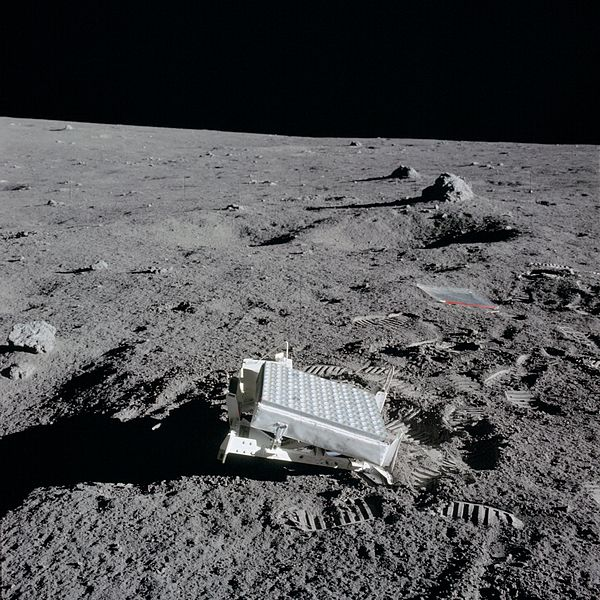
\includegraphics[width=0.3\textwidth]{exercises-2-2}
            \end{center}

            The speed of light is around \SI{3.00}{\metre\per\second}.

    \begin{parts}
      \part Such an experiment finds that the time taken from emission of light to the detection of the reflected pulse is \SI{2.5}{\second}.
            How far away is the moon, approximately?
      \part A 10-cent coin (diameter \SI{20}{\milli\metre}) is found to cover the moon exactly when held at a distance \SI{2.2}{\metre}
            away from the eye. What is the approximate diameter of the moon?
    \end{parts}

  \question Draw an isosceles triangle, with equal sides 1 and included angle $ 2\alpha $; draw the perpendicular line from the included
            angle to the base.
            \begin{center}
              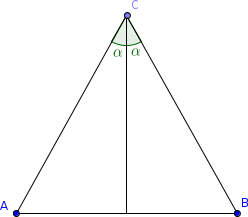
\includegraphics[width=0.3\textwidth]{exercises-2-1}
            \end{center}
            Let $ D $ be the intersection point between $ BC $ and the perpendicular line through $ A $. Show that:
            \begin{itemize}
              \item The base length, $ AB $, is $ 2\sin\alpha $;
              \item The perpendicular segment length, $ AD $, is $ \sin 2\alpha $;
              \item The interior angle at $ B $ is $ \pi/2 - \alpha $.
            \end{itemize}
            Hence, by considering the triangle $ ABD $, show that $ \sin 2\alpha = 2\sin \alpha \cos \alpha $.

  \question We will now generalise question 4. An \emph{isometry} is a mapping $ \iota $ in the plane (i.e. a function taking points
            to points) which preserves lengths; in other words, $ \iota $ is an isometry if for each pair of
            points $ A $ and $ B $, $ \abs{AB} = \abs{\iota(A)\iota(B)} $. (Recall that if $ f $ is a function/map (they mean the same
            thing) then $ f(x) $ denotes the output of $ f $ when fed the input $ x $.)
    \begin{parts}
      \part Let $ X = (x_1, x_2) $ be any point except $ (0,0) $. Define the mapping $ T_X $ to be the function that sends each point $ P = (p_1, p_2) $
            to $ T_X(P) = (p_1 + x_1, p_2 + x_2) $.
        \begin{itemize}
          \item Show that $ T_X $ is an isometry (called the \emph{translation} through $ X $).
          \item Show that there is \textbf{no} point $ F $ such that $ T_X(F) = F $.
          \item Draw the action of $ T_X $ on points in the plane. (`Draw a picture showing what $ T_X $ does.')
        \end{itemize}
      \part Fix some angle $ \theta \neq 0 $. Show that the mapping $ R_\theta $, defined by
            \begin{displaymath}
              R_\theta\left((x,y)\right) = (x \cos \theta - y \sin \theta, x \sin \theta + y \cos \theta)
            \end{displaymath}
            is an isometry. Does there exist any point $ F $ such that $ R_\theta(F) = F $? How many? Draw
            the action of $ F $ on points in the plane.
      \part Let $ \theta $ and $ \phi $ be two angles. Show that
            \begin{displaymath}
              R_\phi\left(R_\theta\left((1,0)\right)\right) = (\cos \theta \cos \phi - \sin \theta \sin \phi, \cos \theta \sin \phi + \sin \theta \cos \phi).
            \end{displaymath}
            By considering the geometric meaning of $ R_\theta $, conclude that $ \cos(\theta + \phi) = \cos \theta \cos \phi - \sin \theta \sin \phi $
            and $ \sin(\theta + \phi) = \cos \theta \sin \phi + \sin \theta \cos \phi $.
            \footnote{Note: a proper proof of this last identity is given as theorem 4.1 in the notes. The issue with this heuristic argument here is that
             we have not got a formal notion of `rotation' that allows us to conclude that if we do a rotation by one angle, followed by
             a rotation by another, then we do indeed get a rotation through the sum of the angles. If we take the above to be the \emph{definition}
             of a rotation, then when we prove this identity using the properties of $ \sin $ and $ \cos $ then we will have \emph{shown}
             that the composition of two rotations is the rotation whose angle is the sum of the first two. Combined with the fact that the map
             is an isometry that fixes a single point,  we will have proved that the map $ R_\theta $ does indeed satisfy all three properties
             that it `should' satisfy in order to be called a rotation. If you don't get what the problem is here, it's not the end of the world,
             it is a little subtle.}
    \end{parts}
\end{questions}

\paragraph{Additional reading} Hobson, chapter III. For a nice treatment of isometries, see Coxeter chapter 3.

\end{document}
